\documentclass[12pt]{article}
\pdfinfoomitdate=1
\pdftrailerid{}
\usepackage[letterpaper,margin=0.65in,headheight=16pt,headsep=20pt,footskip=26pt]{geometry}
\usepackage{tikz}
\usetikzlibrary{arrows.meta}
\usepackage{fancyhdr}
\usepackage[T1]{fontenc}
\usepackage{lmodern}
\renewcommand{\familydefault}{\sfdefault}
\pagestyle{fancy}\fancyhf{}
\fancyhead[L]{\small Week 96 / Prime bags / Grades 4--5}
\fancyfoot[L]{\scriptsize Bellingham Math Circle / Week 96 / W96-45-v2}
\fancyfoot[R]{\small\thepage}
\renewcommand{\headrulewidth}{0.4pt}\renewcommand{\footrulewidth}{0pt}
\setlength{\parindent}{0pt}\setlength{\parskip}{8pt}
\newcommand{\problem}[2]{\par\noindent\textbf{Problem #1:} #2\par}
\newcommand{\card}[1]{\tikz[baseline=(n.base)]\node[draw,rounded corners=2pt,minimum width=1cm,minimum height=.8cm](n){#1};}
\newcommand{\bag}[1]{\begin{tikzpicture}[baseline=(current bounding box.center)]
\draw[rounded corners=9pt](-.5,-.43) rectangle (3.4,.43);
\foreach \v [count=\i from 0] in {#1}{\node[draw,circle,minimum size=.52cm,inner sep=0pt] at (.58*\i,0) {\v};}
\end{tikzpicture}}
\newcommand{\workbox}[2]{\begin{tikzpicture}\draw[gray!65,rounded corners=3pt](0,0) rectangle (#1,#2);\end{tikzpicture}}
\begin{document}
A number card can split into two whole numbers greater than 1 that multiply to its value. These numbers are its factors. Keep splitting until every card is prime: a number greater than 1 that cannot split. The finished cards make a prime bag. Multiply its tokens to find its value.

\begin{center}
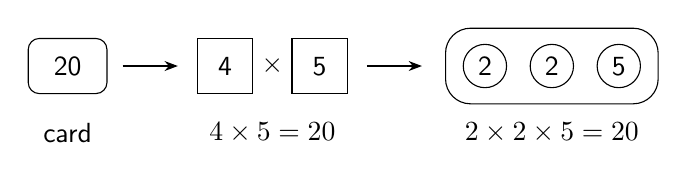
\begin{tikzpicture}[x=1cm,y=1cm,>=Stealth]
\node[draw,rounded corners,minimum width=1cm,minimum height=.7cm] at (0,0){20};
\draw[->] (.7,0)--(1.4,0);
\node[draw,minimum size=.7cm] at (2,0){4};\node at (2.6,0){$\times$};\node[draw,minimum size=.7cm] at (3.2,0){5};
\draw[->] (3.8,0)--(4.5,0);
\draw[rounded corners=9pt](4.8,-.48) rectangle(7.5,.48);
\foreach \v [count=\i from 0] in {2,2,5}{\node[draw,circle,minimum size=.55cm,inner sep=0pt] at(5.3+.85*\i,0){\v};}
\node at (0,-.85){card};\node at (2.6,-.85){$4\times5=20$};\node at (6.15,-.85){$2\times2\times5=20$};
\end{tikzpicture}
\end{center}
Token order does not matter. Tokens with the same number are the same.

\problem{1}{Find different splitting routes for 36, 48 and 60. Can a number have two different finished prime bags?}

\begin{tikzpicture}\draw[gray!65,rounded corners=3pt](2,0) rectangle (17.8,4.2);\node[draw,rounded corners=2pt,minimum width=1cm,minimum height=.8cm] at(.5,2.1){36};\end{tikzpicture}\par
\begin{tikzpicture}\draw[gray!65,rounded corners=3pt](2,0) rectangle (17.8,4.2);\node[draw,rounded corners=2pt,minimum width=1cm,minimum height=.8cm] at(.5,2.1){48};\end{tikzpicture}\par
\begin{tikzpicture}\draw[gray!65,rounded corners=3pt](2,0) rectangle (17.8,4.2);\node[draw,rounded corners=2pt,minimum width=1cm,minimum height=.8cm] at(.5,2.1){60};\end{tikzpicture}\par

\newpage

Choose some tokens from a bag, using each token at most once. The chosen tokens form a bag. You may choose all of them or none. An empty bag has value 1. A divisor of a whole number divides it with no remainder.

\begin{center}
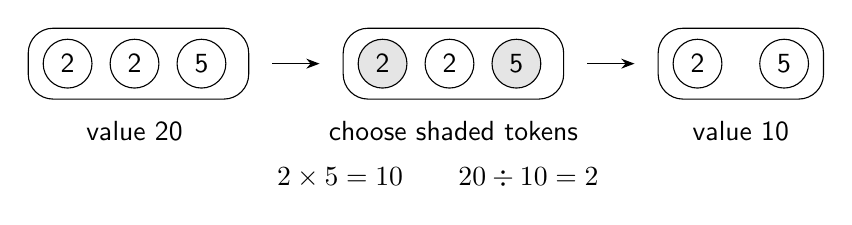
\begin{tikzpicture}[x=1cm,y=1cm,>=Stealth]
\draw[rounded corners=9pt](-.5,-.45) rectangle(2.3,.45);
\node[draw,circle,minimum size=.55cm] at(0,0){2};
\node[draw,circle,minimum size=.55cm] at(.85,0){2};
\node[draw,circle,minimum size=.55cm] at(1.7,0){5};
\draw[->](2.6,0)--(3.2,0);
\draw[rounded corners=9pt](3.5,-.45) rectangle(6.3,.45);
\node[draw,circle,minimum size=.55cm,fill=gray!20] at(4,0){2};
\node[draw,circle,minimum size=.55cm] at(4.85,0){2};
\node[draw,circle,minimum size=.55cm,fill=gray!20] at(5.7,0){5};
\draw[->](6.6,0)--(7.2,0);
\draw[rounded corners=9pt](7.5,-.45) rectangle(9.6,.45);
\node[draw,circle,minimum size=.55cm] at(8,0){2};
\node[draw,circle,minimum size=.55cm] at(9.1,0){5};
\node at(.85,-.85){value 20};\node at(4.9,-.85){choose shaded tokens};\node at(8.55,-.85){value 10};
\node at(4.7,-1.45){$2\times5=10\qquad 20\div10=2$};
\end{tikzpicture}
\end{center}

\problem{2}{For each bag, find every different value you can make by choosing tokens. Explain why your collection is exactly the set of divisors of the full bag's value.}

\bag{2,2,2,3}\quad value 24\par\workbox{17.8}{5.0}\par\bag{2,3,5}\quad value 30\par\workbox{17.8}{5.0}\par

\newpage

\problem{3}{How many different values can you make by choosing tokens from each bag? Find a way to be certain of each total without listing every value.}

\bag{2,2,3,3}\quad value 36\par\workbox{17.8}{3.2}\par\bag{2,2,3,5}\quad value 60\par\workbox{17.8}{3.2}\par\bag{2,2,2,3,3}\quad value 72\par\workbox{17.8}{3.2}\par

\problem{4}{A bag has seven 2 tokens and four 3 tokens. How many different divisors does its value have? Explain a counting rule that works for any prime bag.}

\workbox{17.8}{7.5}

\newpage

\problem{5}{Draw prime bags using any of 2, 3 and 5 whose values have exactly 6, 8, 9, 10 and 12 divisors. Find all possible token-count patterns for each target. A bag with two 2s and one 3 has the same pattern as a bag with two 5s and one 2.}

\vspace{6pt}
6 divisors\par\workbox{17.8}{2.8}

8 divisors\par\workbox{17.8}{2.8}

9 divisors\par\workbox{17.8}{2.8}

10 divisors\par\workbox{17.8}{2.8}

12 divisors\par\workbox{17.8}{2.8}

\newpage

\problem{6}{Find the least positive number with each divisor count below. You may use any primes. Explain how you can rule out every smaller number.}

\vspace{6pt}
4 divisors\par\workbox{17.8}{2.3}

6 divisors\par\workbox{17.8}{2.3}

8 divisors\par\workbox{17.8}{2.3}

9 divisors\par\workbox{17.8}{2.3}

10 divisors\par\workbox{17.8}{2.3}

12 divisors\par\workbox{17.8}{2.3}

\end{document}
